\chapter{Processes of OCR}
\label{ch:tech_stuff}

%-----------------------------------------
% Sections
%-----------------------------------------

The algorithm that is used to develop the OCR software for printed Hindi characters is based on the different geometrical features/shapes of Hindi characters. Input image is parsed into many sub parts/images based on these features. Then other properties such as distribution of points/pixels and edges within each sub image are features used to recognize parsed symbols.

There are mainly four steps performed in any OCR system:- 
\begin{enumerate}
\item Pre Processing 
\item Segmentation 
\item Character Recognition 
\item Post Processing.
\end{enumerate}

\section{Pre Processing}
The pre-processing phase includes the steps that are necessary to bring the input data into an acceptable form for the further phases. The steps are: 
\begin{enumerate}
\item RGB to GRAY
\item Binarization 
\item Noise removal and smoothing 
\item Skew detection and correction
\end{enumerate}

\subsection{GrayScale Conversion}
In the first process, The input is converted in a gray scale image. A gray scale image is an image having BW shades. The image is converted into a grayscale image to further convert it into an BW image. Gray image has shades from black to white.

\subsection{Binarization}
Since the developed system is only able to perform its task only on binarized images, we have to perform the binarization operation before the actual task starts.
Basically in binarization, all the pixels above the threshold value are assigned a particular value for instance 1 and all the values below the threshold value are given the value = 0.
\subsubsection{There are different types of thresholding for binarization:-}
\begin{itemize}
\item Simple thresholding.
\item Otsu's Binarization.
\end{itemize}

\subsection{Smoothing and noise removal:-}
Images do have some stray pixels and some unwanted marks. By using filter noise can be filtered from the image. Smoothing operation in gray image is used for noise reduction and filtering is used for noise removal. Basically there are two types of filters, linear filter and order statistics filter. Order statistics filters are non-linear filters whose response is based on the ranking of the pixel and then replacing the value of the center pixel with the value known by ranking result. The best example of a non-linear filter is a median filter.

\subsubsection{Median Filtering:-}
The median filter is a non-linear digital filtering technique, often used to remove noise from an image. Such noise reduction is a typical pre-processing step to improve the results of the later processing. This is highly effective in removing salt-and-pepper noise.

\subsection{Skew detection and correction:-}
The deviation of the baseline of the text is called skew. During the scanning process, the whole document or a portion of it is fed through the scanner. Our main goal during skewing will be splitting the rotated image into text blocks, and determining the angle from them. We here create two functions, one of determining the skew angle and the other of rotating the image.

What we are trying to do here is to create bounding boxes around the text and then choosing the largest bounding box and then determining the skew angle from the box. The process at first involves finding the areas of text. To make text block detection easier we will invert and maximize the colors of our image, that will be achieved via thresholding. 

\begin{figure}[H]
    \centering
    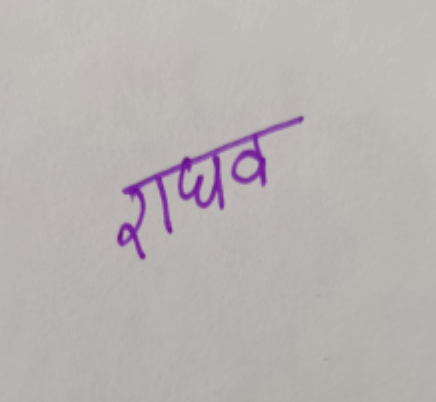
\includegraphics[width=50mm]{figures/image1.png}
    \caption{Before Pre processing}
\end{figure}

\begin{figure}[H]
    \centering
    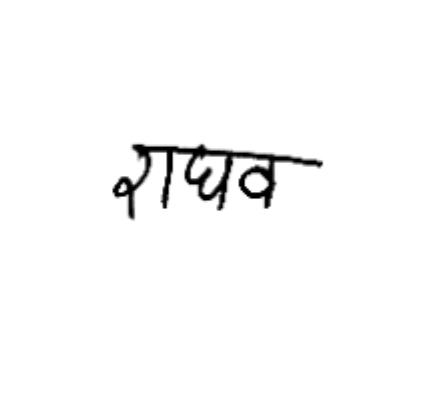
\includegraphics[width=50mm]{figures/image2.png}
    \caption{After Pre processing}
\end{figure}

\newpage

\section{Segmentation}
Segmentation is the way toward parceling a picture/record into disjoint and homogeneous areas. Segmentation is one of the most significant and fundamental procedures that improve the precision pace of character recognition framework. Devanagari report is apportioned into grouping of lines and words by vertical and even projection separately. Process of segmentation involves:-
\begin{enumerate}
\item Segmentation of lines
\item Segmentation of words 
\item Segmentation of characters 
\end{enumerate}

\subsection{Segmentation of lines}
\begin{itemize}
\item A horizontal scanning method is applied for segmenting the text paragraphs into lines. 
\item While performing the segmentation to extract the lines from the text blocks, it performs horizontal scanning starting from the top of the scanned document till it locates the last row containing all white pixels, before a black pixel row is encountered. 
\item It continues the scanning further, till it locates the first row containing all white pixels, just after the end of the last row of black pixels. 
\item This determines a line, and is eventually extracted. This whole process is repeated on the entire text page to segment all the text lines present in that particular page/paragraph.
\end{itemize}

\subsection{Segmentation of Words}
\begin{itemize}
\item After segmenting the lines it segments the individual words embedded in each line.
\item To perform this operation a vertical scanning method is applied. The vertical scanning is applied to the width of the line only. 
\item Analysis of this projection will give us a clear idea about the starting and ending column of each character lying within that text line and amount of space between two adjacent characters.
\end{itemize}

\subsection{Segmentation of Characters}
\begin{itemize}
\item A further segmentation process is applied to achieve the individual characters out of the segmented words. 
\item Before segmenting words at character level, the header line or shirorekha is identified and removed. 
\item Once the shirorekha is properly removed, the word is divided into three horizontal zones known as upper, middle and lower zones. Individual characters are separated from each zone by applying vertical scanning
\end{itemize}


\section{Character Recognition}
After the extraction of individual characters occurs, a recognition engine is used to identify the corresponding computer character. Several different recognition techniques are currently available.

\subsection{K-Nearest Neighbor(KNN) Algorithm for Machine Learning:-}
\begin{itemize}
\item K-Nearest Neighbour is one of the simplest Machine Learning algorithms based on Supervised Learning technique.
\item The K-NN algorithm assumes the similarity between the new case/data and available cases and puts the new case into the category that is most similar to the available categories.
\item KNN algorithm is used for classification (most commonly) and regression. It is a versatile algorithm also used for imputing missing values and resampling datasets.
\item There are three limitations of KNN:-
\begin{itemize}
\item When K is greater than one and if numbers of train samples of different classes are the same then there will be a tie for assignment of a specific class.
\item When any input vector (test sample) is assigned to a class, it does not indicate intensity of the vector to that class.
\item All classes are considered with equal strength in assignment of the class label to the test sample.
\end{itemize}
\item Fuzzy KNN:-
\begin{itemize}
\item To avoid the above mentioned disadvantages of KNN algorithm, fuzzy set concept is introduced into it.
\item The Fuzzy K-Nearest Neighbor algorithm assigns class membership to a test sample rather than defining specific class.
\end{itemize}
\end{itemize}

\subsection{Convolutional Recurrent Neural Network:-}
\begin{itemize}
\item The Convolutional Recurrent Neural Networks is the combination of two of the most prominent neural networks. The CRNN (convolutional recurrent neural network) involves CNN(convolutional neural network) followed by the RNN(Recurrent neural networks).
\item We use CRNN to extract the important features from the handwritten line text Image.
\item Most of the time, the Convolutional Neural Network analyzes the image, sending it to the recurrent part of the important features detected.
\item The recurrent part analyzes these features in order, taking into consideration previous information in order to realize what are some important links between these features that influence the output.
\end{itemize}

\subsection{Connectionist Temporal Classification (CTC):-}
The NN outputs character-scores for each sequence-element, which simply is represented by a matrix. Now, there are two things we want to do with this matrix:
\begin{itemize}
\item Train: calculate the loss value to train the NN
\item Infer: decode the matrix to get the text contained in the input image
\end{itemize}
Both tasks are achieved by the CTC operation.

\begin{figure}[H]
    \centering
    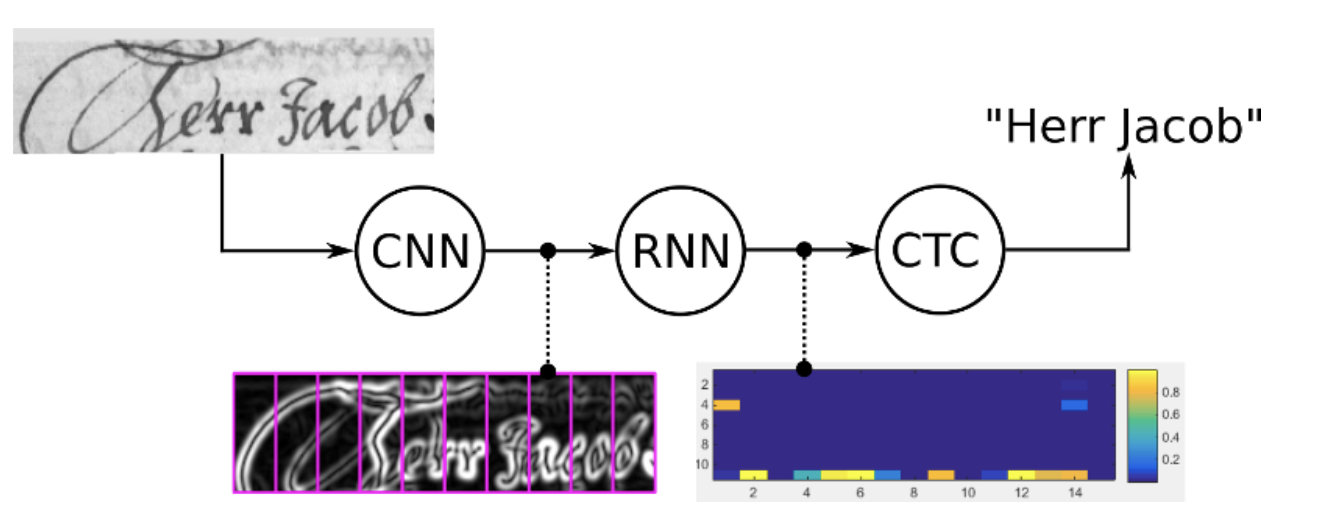
\includegraphics[width=150mm]{figures/image3.png}
\end{figure}

The NN-training will be guided by the CTC loss function. We only feed the output matrix of the NN and the corresponding ground-truth (GT) text to the CTC loss function.

\section{Post Processing}
Post-handling stage is the last phase of the proposed recognition framework. The post processing phase includes the conversion of the UNICODE in to standard output into any standard text encoding scheme.

\begin{figure}[H]
    \centering
    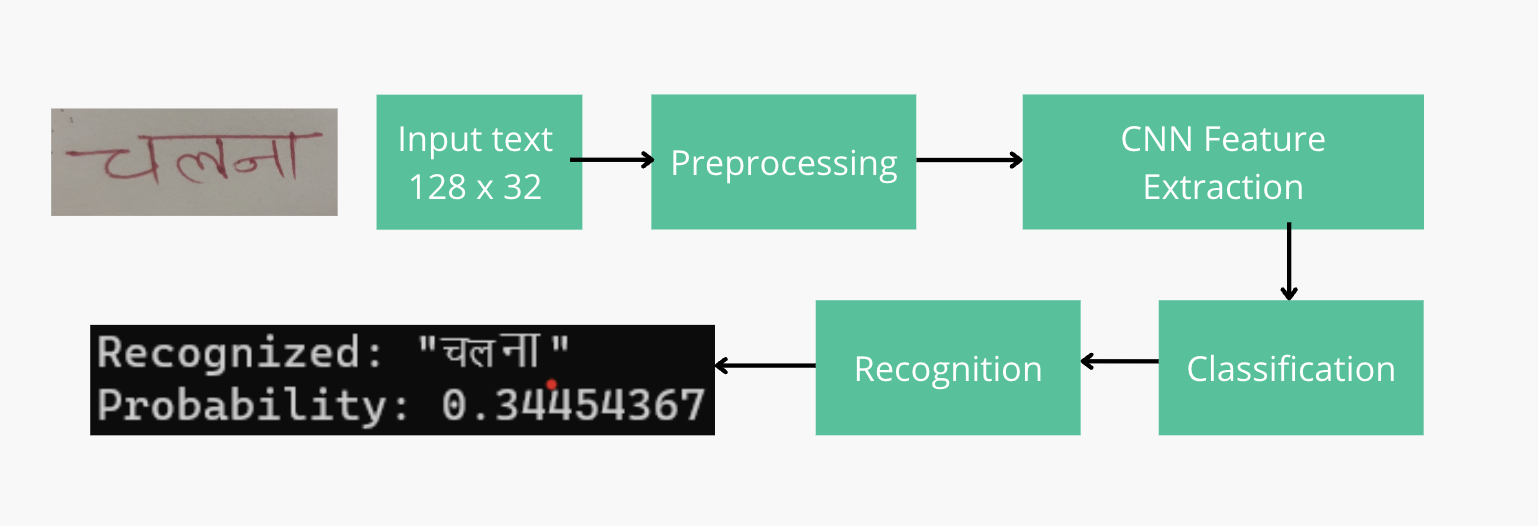
\includegraphics[width=150mm]{figures/image4.png}
    \caption{The Complete process of an OCR}
\end{figure}